\documentclass[a4paper,12pt]{article}
%%%%%%%%%%%%%%%%%%%%%%%%%%%%%%%%%%%%%%%%%%%%%%%%%%%%%%%%%%%%%%%%%%%%%%%%%%%%%%%%%%%%%%%%%%%%%%%%%%%%%%%%%%%%%%%%%%%%%%%%%%%%%%%%%%%%%%%%%%%%%%%%%%%%%%%%%%%%%%%%%%%%%%%%%%%%%%%%%%%%%%%%%%%%%%%%%%%%%%%%%%%%%%%%%%%%%%%%%%%%%%%%%%%%%%%%%%%%%%%%%%%%%%%%%%%%
\usepackage{eurosym}
\usepackage{vmargin}
\usepackage{amsmath}
\usepackage{graphics}
\usepackage{epsfig}
\usepackage{subfigure}
\usepackage{fancyhdr}
\usepackage{listings}
\usepackage{framed}
\usepackage{graphicx}
\usepackage{amsmath}
\usepackage{chngpage}
%\usepackage{bigints}


\setcounter{MaxMatrixCols}{10}
%TCIDATA{OutputFilter=LATEX.DLL}
%TCIDATA{Version=5.00.0.2570}
%TCIDATA{<META NAME="SaveForMode" CONTENT="1">}
%TCIDATA{LastRevised=Wednesday, February 23, 2011 13:24:34}
%TCIDATA{<META NAME="GraphicsSave" CONTENT="32">}
%TCIDATA{Language=American English}

%\pagestyle{fancy}
%\setmarginsrb{20mm}{0mm}{20mm}{25mm}{12mm}{11mm}{0mm}{11mm}
%\lhead{MA4413} \rhead{Mr. Kevin O'Brien}
%\chead{Statistics For Computing}
%\input{tcilatex}

\begin{document}
\begin{center}
       
\includegraphics[scale=0.55]{shieldtransparent2}
\end{center}

\begin{center}
\vspace{1cm}
\large \bf {FACULTY OF SCIENCE AND ENGINEERING} \\[0.5cm]
\normalsize DEPARTMENT OF MATHEMATICS AND STATISTICS \\[1.25cm]
\large \bf {MID-SEMESTER ASSESSMENT} \\[1.5cm]
\end{center}

\begin{tabular}{ll}
MODULE CODE: MA4128 & SEMESTER: Spring \\[1cm]
MODULE TITLE: Advanced Data Modeling & DURATION OF EXAM: 1 hour \\[1cm]
LECTURER: Mr. Kevin O'Brien & GRADING SCHEME: 50 marks \\
& \phantom{GRADING SCHEME:} \footnotesize {20\% of module grade} \\[0.8cm]
\\[1cm]
\end{tabular}
\begin{center}
{\bf INSTRUCTIONS TO CANDIDATES}
\end{center}

{\noindent \\ Scientific calculators approved by the University of Limerick can be used. \\
Statistical tables provided at the end of the exam paper.\\
Students must attempt ALL questions}
\newpage



% - Section 1 Inference Procedures
        % a. Parametric
        % b. Non Parametric
% - Section 2 Linear Models
        % a. SLR
        % b. MLR
% - Section 3 Linear Models
        % a. Robust Regression
        % b. AIC
% - Section 4 Statistical Process control
        % a. Control Limits
        % b. Theory Questions
        % c. Interpreting Charts
        % d. CUSUM and ARL
% - Section 5 Experimental Design 1
        % a. Definitions for ED
        % b. One Way ANOVA
% - Section 6 Experimental Design 2
        % a.
        % b.


\subsection*{Question 1. (10 marks) Distributional Assumptions}
\begin{itemize}
\item[(a)] (5 Marks) 

The data set \texttt{X} and \texttt{Y} are both assumed to be normally distributed. The Shapiro-Wilk test was carried out to assess whether or not this assumption is valid for data set \texttt{X}.
\begin{itemize}
	\item[(i.)] (1 Mark) Formally state the null and alternative hypothesis.
	\item[(ii.)] (2 Marks) What is your conclusion for this procedure? Justify your answer.
\end{itemize}
\begin{framed}
\begin{verbatim}
> shapiro.test(X)
	
Shapiro-Wilk normality test
data:  X
W = 0.9292, p-value = 0.372
\end{verbatim}
\end{framed}

 Continuing with the data sets \texttt{X} and \texttt{Y}, graphical procedure was carried out to assess whether or not this assumption of normality is valid for data set \texttt{Y}. Consider the Q-Q plot in the figure below.

\begin{center}
	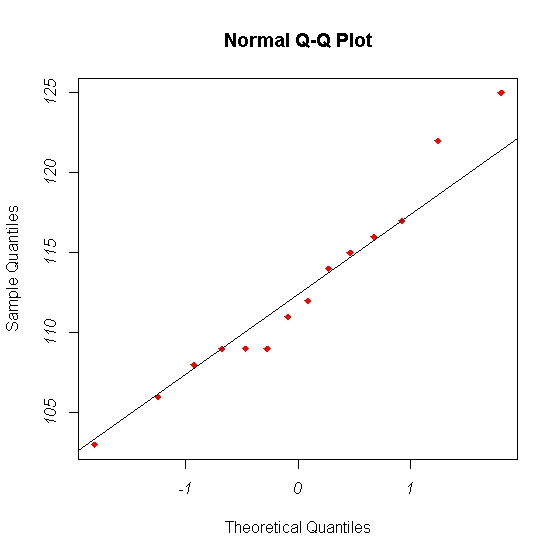
\includegraphics[scale=0.45]{Q5examQQplot}
\end{center}

\begin{itemize}
	\item[(iii.)] (1 Mark) Provide a brief description on how to interpret this plot.
	\item[(iv.)] (1 Mark) What is your conclusion for this procedure? Justify your answer.
\end{itemize}

\item[(b)] (5 Marks) 

The typing speeds for one group of 10 Engineering students were recorded both at the beginning of year 1 of their studies. The results (in words per minute) are given below:

\begin{center}
	\begin{tabular}{|c|c|c|c|c|}
		\hline
		% Subject& A& B& C& D& E &F &G &H \\ \hline
		149  & 146 & 122 & 142 &  153\\ \hline
		137 & 151 & 156&   170&  149
		\\ \hline
	\end{tabular}
\end{center}
Use the Dixon Q-test to determine if there is an outlier present in this data. You may assume a significance level of 5\%. Critical values are tabulated at the back of this exam paper.
\begin{itemize}
	\item[(i.)](1 Mark)	State the null and alternative Hypothesis for this test.
	\item[(ii.)](1 Mark) Compute the test statistic
	\item[(iii.)](1 Mark) State the appropriate critical value.
	\item[(iv.)](1 Mark) What is your conclusion to this procedure.
	\item[(v.)] (1 Mark ) Briefly discuss any limitations upon using this test.
\end{itemize}
\end{itemize} 
%--------------------------------------------------------------------------------------------------------%


\newpage
\subsection*{Question 2. (10 marks) Binary Classification }
%\subsection*{Question 4. (20 marks) }


\end{itemize}


%-------------------------------Start of Question 2A%
\newpage







%%-------------------------------------%
%\subsection*{Question 3. (20 marks) Multiple Linear Regression Models }
%\begin{itemize}
%
%\item[(a)] Explain the following terms:
%\begin{itemize}
%\item[i.] (2 marks) Over-fitting,
%\item[ii.] (2 marks) Multicollinearity,
%\item[iii.] (2 Marks) Heteroscedascity.
%\end{itemize}
%\item[(b)] Answer the following questions related to model selection techniques for linear models.
%\begin{itemize}
%\item[i.] (2 marks) Explain why the adjusted $R^2$ value may differ in value from the corresponding multiple $R^2$ value for the same fitted model.
%\item[ii.] (2 marks) Explain how the \emph{Akaike information criterion} would used to compare two models fitted for the same data.
%\end{itemize}
%
%\item[(c)]
%In an experiment to determine hydrolysable tannins in plants by absorption spectroscopy, the following results from ten samples were obtained and are tabulated below. A simple linear regression model, predicting absorbance values using concentration as the independent variable, was fitted to the data.
%
%
%%Absorbance= c(0.084, 0.183, 0.326, 0.464, 0.643, 0.707, 0.717, 0.734 ,0.749 ,0.732) ;
%%Concentration= c(0.123, 0.288, 0.562, 0.921, 1.420, 1.717, 1.921, 2.137 ,2.321, 2.467) ;
%%plot(Concentration,Absorbance,pch=18,col="red",font.axis=2,font.lab=2)
%%abline(coef(lm(Absorbance~Concentration)))
%%
%%Conc.Squared = (Concentration^2)
%%Conc.Cubed = (Concentration^3)
%%ModelA = lm(Absorbance~Concentration)
%%ModelB = lm(Absorbance~Concentration+Conc.Squared)
%%ModelC = lm(Absorbance~Concentration+Conc.Squared+Conc.Cubed)
%
%\begin{center}
%\begin{tabular}{|c||c|c|c|c|c|}
%  \hline
%  % after \\: \hline or \cline{col1-col2} \cline{col3-col4} ...
%Sample & 1 & 2 & 3 & 4 & 5 \\ \hline
%Absorbance & 0.084& 0.183& 0.326& 0.464& 0.643\\
%Concentration & 0.123& 0.288& 0.562& 0.921& 1.420\\ \hline
%Sample & 6 & 7 & 8 & 9 & 10 \\ \hline
%Absorbance & 0.707& 0.717& 0.734 &0.749 &0.732\\
%Concentration & 1.717& 1.921& 2.137 &2.321&2.467\\
%  \hline
%\end{tabular}
%\end{center}
%
%\begin{center}
%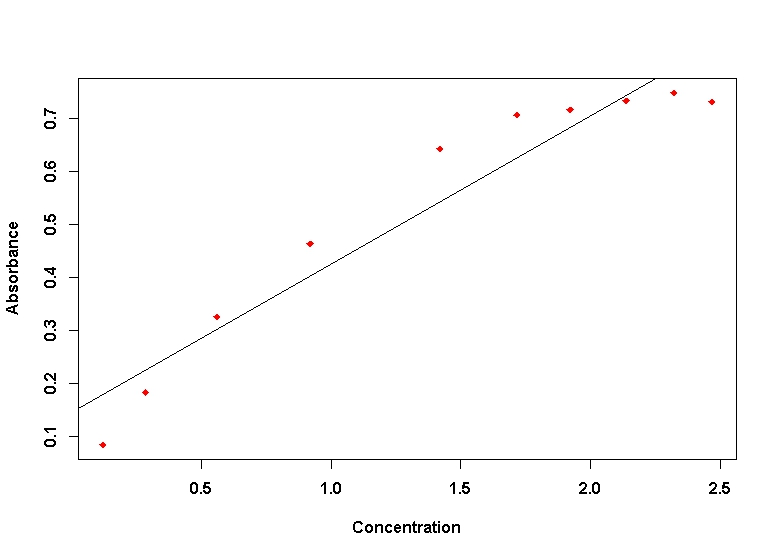
\includegraphics[scale=0.55]{ExamQ3plot}
%\end{center}
%
%
%\begin{itemize}
%\item[i.] (2 marks) Is the simple linear regression model approach suitable for this study? Explain your answer with reference to the scatter-plot.
%%\item[ii] (2 marks) Two polynomial models were also fitted to the data. Description of all three fitted models are found in the three blocks of \texttt{R} code below. The \emph{Akaike information criterion} is also listed, for each of the three fitted models.
%\end{itemize}
%
%
%
%\item[(d)] 
%
%%\end{document}
%--------------------------------------------------------%

\subsection*{Question 3. (10 marks) Hierarchical Clustering}


\begin{itemize}
		\item[(i.)](1 Mark)  Compute the Euclidean distance between the following points.
		\[ A = \c(4,6,8,2)\]
		\[ B = \c(3,6,1,6)\]
%		
%	\item[(i.)](2 Marks) What is the purpose of a cluster analysis?
	
%	\item[ii.](2 Marks)  A discriminant analysis is similar to a cluster analysis; however, there is one fundamental difference.  Explain this difference.
	
	\item[(ii.)](2 Marks) Why do you standardize variables before carrying out a cluster analysis.
		Explain why using the standardized value may not be suitable in some cases? Give another example of numeric transformation. 
	%What is the difference between a linkage method and a distance measure?
	
	\item[(iii.)](4 Marks)  Compare and contrast any three linkage methods. Support your answer with sketches
	
	\item[(iv.)](1 Mark)  In the context of hierarchical cluster analysis, distinguish between agglomerative clustering and divisive clustering.
	%	\item[ix.](2 Marks)  What is a vertical icicle plot used for? Give a brief description, supporting your answer with sketches.

	
	
	\item[(v.)](2 Marks)  How do we determine the appropriate number of clusters?  Give two different visualization methods that are used to display the outcome of a cluster analysis.
	
%	\item[vi.](2 Marks) Standardization
%	
%	\item[vii.](2 Marks)  Explain the difference between Ward's method and k-means
%	clustering.
%	%\item[7.] Vertical Icicle Plot


	
\end{itemize}



%-----------------------------------------------------------%
\newpage

\subsection*{Question 4. (10 marks) K-Means Clustering}

\begin{itemize}
	\item[(i.)] (5 Marks) Explain the process of k-means clustering, starting with initial cluster allocation. You may work on the basis of a two-cluster solution. Support your answer with several sketches.
	\item[(ii.)] (2 Marks) Compare and contrast k-means clustering and hierarchical clustering in terms of the number of cluster determined.
	\item[(iii.)] (3 Marks) For a 4 cluster solution, Interpret the ANOVA table below.
\end{itemize}


\begin{figure}[h!]
\centering
\includegraphics[width=1.1\linewidth]{ANOVA}
\end{figure}



%------------------------------------------------------------------------ %
\Large{
\newpage
	\section*{Formulas and Tables}
	
	\subsection*{Critical Values for Dixon Q Test}
	{
		\Large
		\begin{center}
			\begin{tabular}{|c|c|c|c|}
				\hline  N  & $\alpha=0.10$  & $\alpha=0.05$  & $\alpha=0.01$  \\ 
			    &{\normalsize \textit{Confidence}$=0.90$ } & {\normalsize \textit{Confidence}$=0.95$ }  & {\normalsize \textit{Confidence}$=0.99$ }   \\ \hline
				3  & 0.941 & 0.97  & 0.994 \\ \hline
				4  & 0.765 & 0.829 & 0.926 \\ \hline
				5  & 0.642 & 0.71  & 0.821 \\ \hline
				6  & 0.56  & 0.625 & 0.74  \\ \hline
				7  & 0.507 & 0.568 & 0.68  \\ \hline
				8  & 0.468 & 0.526 & 0.634 \\ \hline
				9  & 0.437 & 0.493 & 0.598 \\ \hline
				10 & 0.412 & 0.466 & 0.568 \\ \hline
				11 & 0.392 & 0.444 & 0.542 \\ \hline
				12 & 0.376 & 0.426 & 0.522 \\ \hline
				13 & 0.361 & 0.41  & 0.503 \\ \hline
				14 & 0.349 & 0.396 & 0.488 \\ \hline
				15 & 0.338 & 0.384 & 0.475 \\ \hline
			\phantom{sp}	16 \phantom{sp} & 0.329 & 0.374 & 0.463 \\ \hline
			\end{tabular} 
		\end{center}
	}
	


\end{document}




